\documentclass{article}

\usepackage[T1]{fontenc}
\usepackage[utf8]{inputenc}

\usepackage{amsmath, amssymb, amsfonts}
\usepackage[margin=3cm]{geometry}
\usepackage{listings}
\usepackage{graphicx}
\usepackage{enumerate}

\begin{document}
    \section*{Problem 1}
        \begin{enumerate}[(i)]
            \item Comparison between Theorem 4.18 and Theorem 4.7: For the steepest descent method (GD), we have a worst case convergence result for every single step. This is due to the fact that the method has no memory and each step is therefore independent of the other steps.
            The conjugate gradient method (CG), on the other hand, gives a result that holds only globally, for $k$ steps. Therefore, we have Q-linear convergence for GD, while we have only R-linear convergence for the CG.
            In both cases, however, the objective values and, as a result, the norm of the error are monotonically decreasing.
            For $k$ steps, the convergence factor for CG (considering the objective values) is
            \[
                2 \left(\frac{\sqrt{\kappa} - 1}{\sqrt{\kappa} + 1}\right)^{2k},
            \]
            i.e. in order to reduce the initial error by a factor of $\varepsilon$, it takes
            \[
                k \leq \left\lceil\frac{\sqrt{\kappa}}{4}\ln\left(\frac{2}{\varepsilon}\right)\right\rceil
            \]
            steps.
            For $k$ steps, the convergence factor for GD (considering the objective values) is
            \[
                \bigl(\frac{\kappa - 1}{\kappa + 1}\bigr)^{2k},
            \]
            i.e. in order to reduce the initial error by a factor of $\varepsilon$, it takes
            \[
                k \leq \left\lceil\frac{\kappa}{4}\ln\left(\frac{1}{\varepsilon}\right)\right\rceil
            \]
            steps.
            \item We use gnuplot, 
            \[
                \lstinline|plot [1:100] kappa/4*6*log(10), sqrt(kappa)/4*6*log(20)|
            \]
            and get
            \begin{center}
                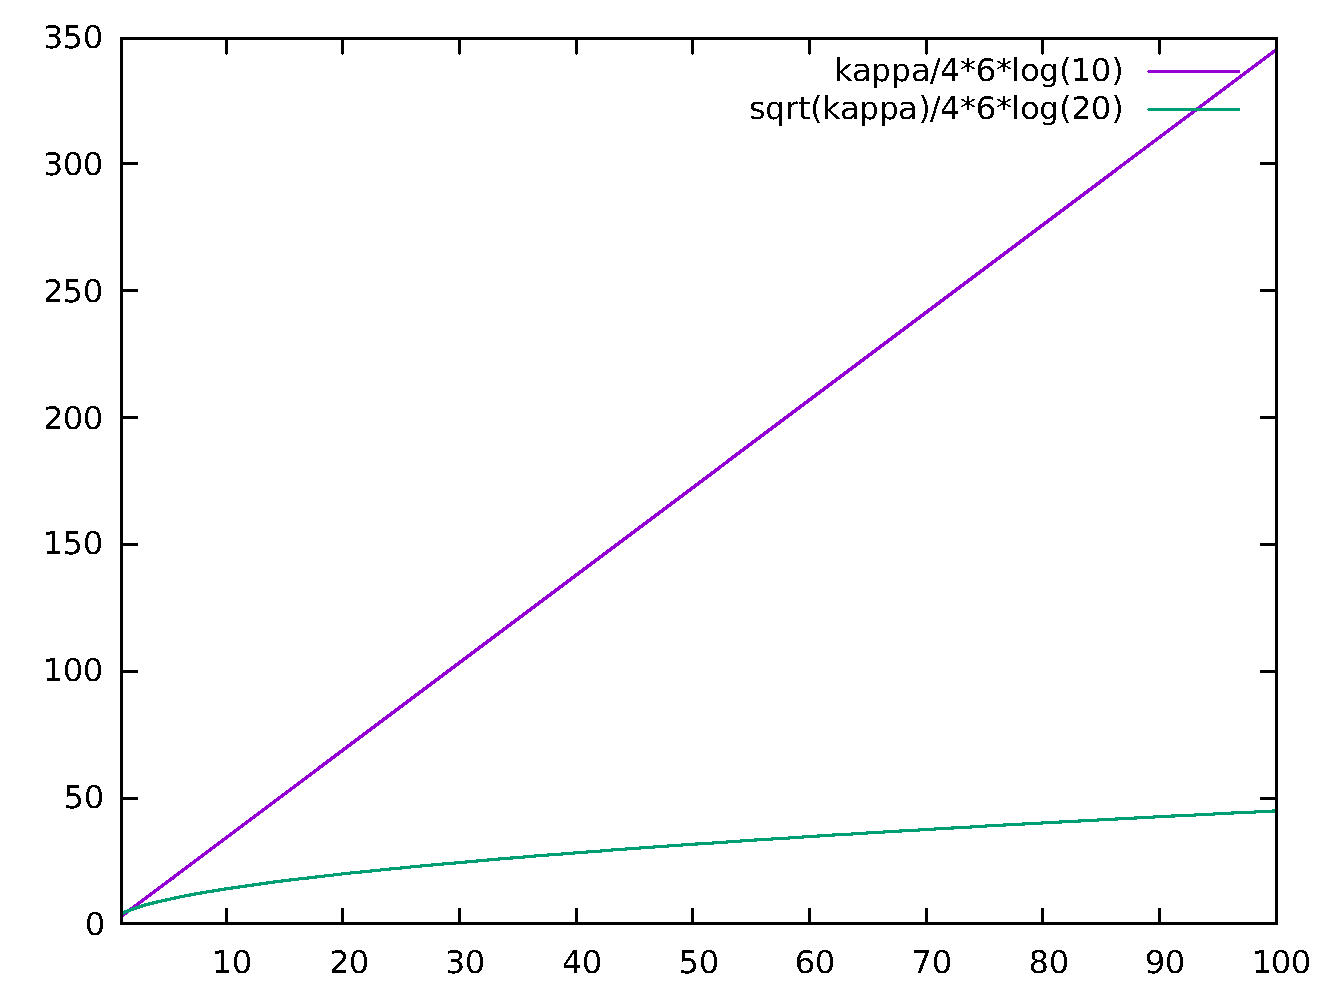
\includegraphics[width=0.8\textwidth]{1_ii.pdf}
            \end{center}
        \end{enumerate}
    \section*{Problem 2}
    We have
    \[
        \tilde x^{(k+1)} - x^{(k+1)} = - \alpha^{(k)}\beta^{(k)}d^{(k-1)}.
    \]
    Because of Lemma 4.14, we know that with the CG method we would converge within at most $n$ steps. 
    \[
        x^{(k+1)} - x^*= \sum_{i=k+1}^{n-1} \gamma_i d^{(i)}
    \]
    for some scalars $\gamma_i$. All involved directions $d^{(i)}$ are $A$-conjugate to any previous direction, in particular we have 
    \[
        d^{(k-1), \top} A \left(x^{(k+1)} - x^*\right) = 0.
    \]
    As a result,
    \begin{align*}
        \lVert \tilde x^{(k+1)} - x^* \rVert _A 
        &= \lVert \tilde x^{(k+1)} - x^{(k+1)} + x^{(k+1)} - x^* \rVert _A\\
        &= \left(- \alpha^{(k)}\beta^{(k)}d^{(k-1)} + x^{(k+1)} - x^* , - \alpha^{(k)}\beta^{(k)}d^{(k-1)} + x^{(k+1)} - x^*\right) _A\\
        &= \lVert - \alpha^{(k)}\beta^{(k)}d^{(k-1)}\rVert _A + \lVert x^{(k+1)} - x^*\rVert _A\\
        &\geq \lVert x^{(k+1)} - x^*\rVert _A.
    \end{align*}
    \section*{Problem 3}
    First, we show that the number of steps is bounded by the dimension of
    \[
        S := \operatorname*{span}\left(r^{(0)}, \dots, (AM^{-1})r^{(0)}\right).  
    \]
    
    \[
        A = MV\Lambda V^\top M \text{ und daher } AM^{-1} = MV\Lambda V^\top.  
    \]
    Insbesondere erhalten wir 
\end{document}